\documentclass[12pt,aspectratio=169]{beamer}

\usetheme[progressbar=frametitle, numbering=none]{metropolis}
\renewcommand{\emph}[1]{{\color{mLightBrown}#1}}

\usepackage{booktabs}
\usepackage{geometry}
\usepackage{listings}

\graphicspath{{fig/}}

\lstset{%
  basicstyle=\small\ttfamily,
  language={bash},
  breaklines=true,
  emph={$},
  emphstyle={\color{mLightGreen}}, 
}

\usepackage{tikz}
\usetikzlibrary{shapes,arrows}

\tikzstyle{block} = [rectangle, draw,
    text width=5em, text centered, rounded corners, minimum height=4em]

\title{Hashing algorithms \& password cracking}
\author{Jack Walton}
\date{\today}
\institute{Newcastle University}

\begin{document}

\maketitle

\begin{frame}{Table of contents}
\vspace*{\fill}
1. Hash functions\\[4mm]
2. Password Cracking\\[4mm]
3. Setting secure passwords\\[4mm]
4. Cake
\vfill
\end{frame}

\section{Hash functions}

\begin{frame}{Definition}
A hash function $H$ maps from data of \emph{arbitrary size} (the input) to data of \emph{fixed size} (the hash)

Hash functions are designed to be \emph{``one-way''} (easy to compute, hard to invert) 

Toy hash function:
\begin{equation*}
	y = H(x) = \lfloor 5x \text{ mod } 10 \rfloor,\, x\in\mathbb{R} \text{ and } y\in\{0,1,\ldots,9\}
\end{equation*}
\end{frame}

\begin{frame}{Toy function}
Toy hash function:
\begin{equation*}
	y = H(x) = \lfloor 5x \text{ mod } 10 \rfloor,\, x\in\mathbb{R} \text{ and } y\in\{0,1,\ldots,9\}
\end{equation*}
\begin{table}[h]
	\begin{tabular}{@{}cc@{}}
	\toprule
	$x$    & $H(x)$ \\\midrule
	$3.14$ & $5$ \\
	$2.72$ & $3$ \\
	$1.41$ & $7$ \\\bottomrule
	\end{tabular}
	\caption{Input and output values}
\end{table}
\end{frame}

\begin{frame}{Toy usage}
\begin{itemize}
	\item Alice \& Bob are working on a homework problem
	\item They want to check they got the same result
	\item However, they do not want to reveal their answers to one-another
	\item Solution? \onslide<2->{\emph{Hash and compare}}
\end{itemize}
\end{frame}

\begin{frame}{IRL usage: message authentication}
\begin{figure}
	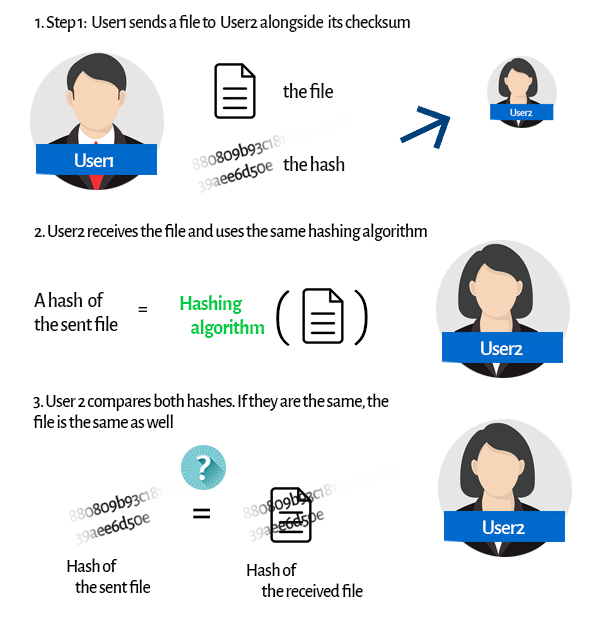
\includegraphics[width=0.5\textwidth]{hashing.png}
\end{figure}
\end{frame}


\begin{frame}{IRL usage: password verification}
\begin{itemize}
	\item Hashes are used to store passwords online
	\item Omits need for developers to store passwords in plaintext
\end{itemize}
\vspace{-0.2cm}
\begin{figure}[h]
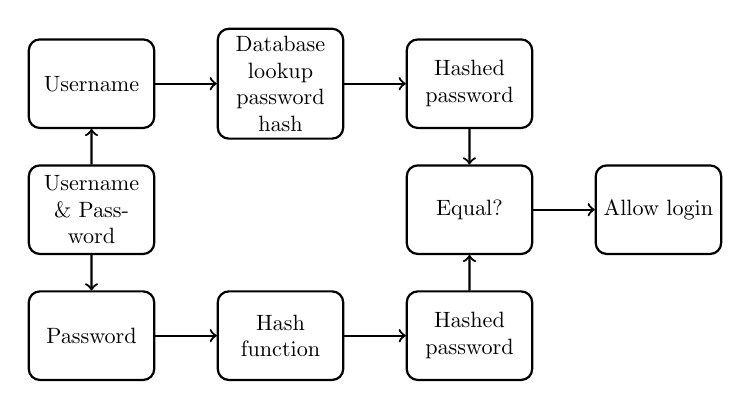
\begin{tikzpicture}[thick, every node/.style={scale=0.8}]
	\node [block] (init) {Username \& Password};
	\node [block, below of=init, node distance=2cm] (pass) {Password};	
	\node [block, above of=init, node distance=2cm] (user) {Username};
	\node [block, right of=user, node distance=3cm] (lookup) {Database lookup password hash};
	\node [block, right of=pass, node distance=3cm] (hash) {Hash function};
	\node [block, right of=hash, node distance=3cm] (hashhashed) {Hashed password};
	\node [block, right of=lookup, node distance=3cm] (dbhashed) {Hashed password};
	\node [block, below of=dbhashed, node distance=2cm] (equal) {Equal?};
	\node [block, right of=equal, node distance=3cm] (login) {Allow login};

        \draw[->] (init) -- (pass);
        \draw[->] (init) -- (user);
        \draw[->] (user) -- (lookup);
        \draw[->] (pass) -- (hash);
        \draw[->] (lookup) -- (dbhashed);
        \draw[->] (hash) --(hashhashed);
        \draw[->] (dbhashed) -- (equal);
        \draw[->] (hashhashed) -- (equal);
        \draw[->] (equal) -- (login);
\end{tikzpicture}
\end{figure}
\end{frame}

\begin{frame}{Desirable properties}
To use hash functions in the wild, we desire them to be:
\begin{enumerate}
	\item Deterministic
	\item Quick to compute given any input
	\item One-way
	\item Very sensitive to input
	\item Infeasible to find collisions
\end{enumerate}
\end{frame}

\begin{frame}{Hashing in the wild: SHA-1}
\begin{itemize}
	\item Designed by the NSA and published in 1995
	\item Produces 160-bit hash (typically rendered as a hexadecimal number)
	\item Not considered secure against well-funded opponents (since 2005)
	\item In 2017 Google performed a \emph{collision attack} on SHA-1
\end{itemize}
\end{frame}

\begin{frame}{IRL usage: message authentication}
\begin{figure}
	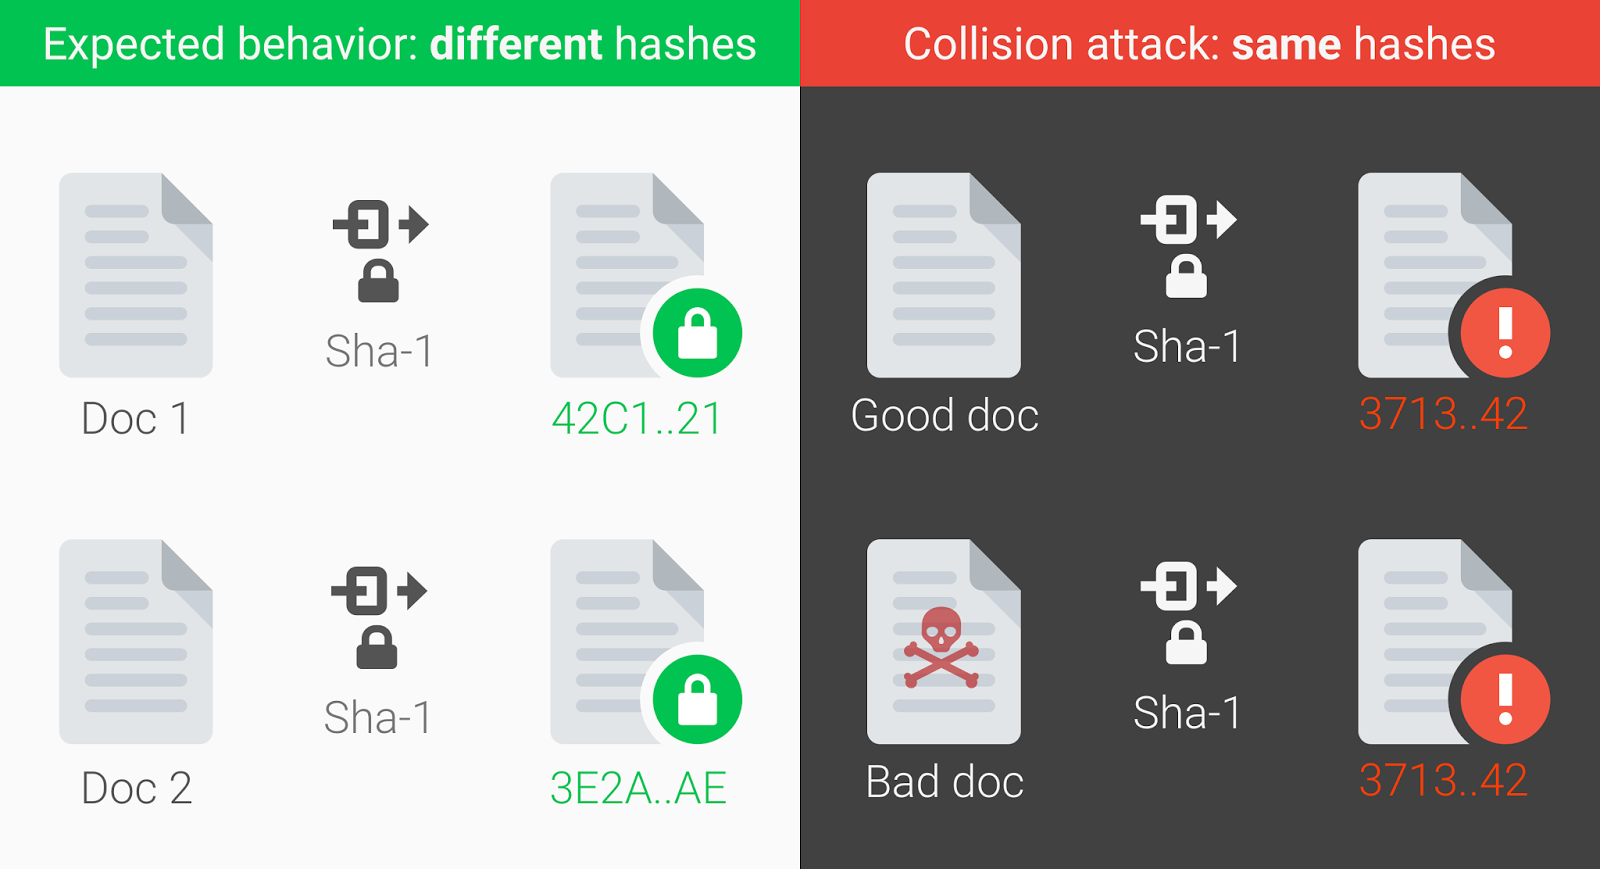
\includegraphics[width=0.85\textwidth]{hash_collision.png}
\end{figure}
\end{frame}

\begin{frame}{Hashing in the wild: SHA-1}
\begin{figure}
    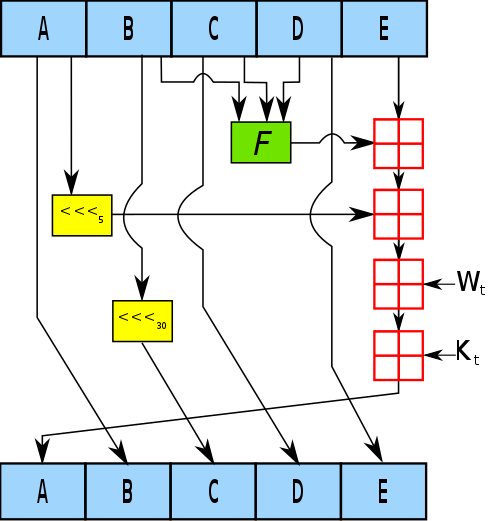
\includegraphics[width=0.5\textwidth]{sha1.png}
\end{figure}
\end{frame}

\begin{frame}{Hashing in the wild: SHA-1}
SHA1("The quick brown fox jumps over the lazy \emph{dog}")
output: 2fd4e1c67a2d28fced849ee1bb76e7391b93eb12

SHA1("The quick brown fox jumps over the lazy \emph{cog}")
output: de9f2c7fd25e1b3afad3e85a0bd17d9b100db4b3
\end{frame}

\section{Password cracking}

\begin{frame}{Hashcat}
	\begin{itemize}
		\item Hashcat advertises as ``World's fastest password cracker''
                \item Cracks passwords from leaked lists of hashed passwords
		\item Cracked passwords \& emails used to attempt access to other services
        \end{itemize}
	\vspace{-0.1cm}
\begin{figure}[h]
    \begin{tikzpicture}[thick, every node/.style={scale=0.8}]
	\node [block] (init) {Username \& Password};
	\node [block, below of=init, node distance=2cm, fill=mLightBrown] (pass) {Password};	
	\node [block, above of=init, node distance=2cm] (user) {Username};
	\node [block, right of=user, node distance=3cm] (lookup) {Database lookup password hash};
	\node [block, right of=pass, node distance=3cm, fill=mLightBrown] (hash) {Hash function};
        \node [block, right of=hash, node distance=3cm, fill=mLightBrown] (hashhashed) {Hashed password};
	\node [block, right of=lookup, node distance=3cm, fill=mLightBrown] (dbhashed) {Hashed password};
        \node [block, below of=dbhashed, node distance=2cm, fill=mLightGreen] (equal) {Equal?};
	\node [block, right of=equal, node distance=3cm] (login) {Allow login};

        \draw[->] (init) -- (pass);
        \draw[->] (init) -- (user);
        \draw[->] (user) -- (lookup);
        \draw[->] (pass) -- (hash);
        \draw[->] (lookup) -- (dbhashed);
        \draw[->] (hash) --(hashhashed);
        \draw[->] (dbhashed) -- (equal);
        \draw[->] (hashhashed) -- (equal);
        \draw[->] (equal) -- (login);
\end{tikzpicture}
\end{figure}
\end{frame}

\begin{frame}{Demonstrations}
    \begin{itemize}
        \item We will use the GPU equipped machine ``Langkawi'' (thanks NPP) to run hashcat
        \item Langkawi is equipped with a NVIDIA Tesla K40c graphics card, with 12gb onboard RAM
	\item Attempt to crack \emph{md5 hashed} passwords released from LulzSec's 2011 hack of EA's Battlefield Heroes game
    \end{itemize}
\end{frame}

\begin{frame}{Brute force demo}
    \lstinline|$ hashcat -m 0 -a 3 -O bfield.hash|
\end{frame}

\begin{frame}{Brute force attack}
	\begin{table}
		\begin{tabular}{p{10.5cm}}
			\toprule
			\centering{Password length}
		\end{tabular}
		\begin{tabular}{@{} l p{1.2mm}p{1.2mm}p{1.2mm}p{1.2mm} p{0.1mm}}
			   & \multicolumn{4}{c}{6} & \\
			   & y & d & h & m & \\\midrule
			26 & 0 & 0 & 0 & 0 & \\
			36 & 0 & 0 & 0 & 0 & \\
			62 & 0 & 0 & 0 & 0 & \\
			95 & 0 & 0 & 0 & 3 & \\\bottomrule
		\end{tabular}%
		\begin{tabular}{p{1.2mm}p{1.2mm}p{1.2mm}p{1.2mm} p{0.1mm}}
			\multicolumn{4}{c}{7} & \\
			y & d & h & m & \\\midrule
			0 & 0 & 0 & 0 & \\
			0 & 0 & 0 & 0 & \\
			0 & 0 & 0 & 14 & \\
			0 & 0 & 4 & 50 & \\\bottomrule
		\end{tabular}%
		\begin{tabular}{p{1.2mm}p{1.2mm}p{1.2mm}p{1.2mm} p{0.1mm}}
			\multicolumn{4}{c}{8} & \\
			y & d & h & m & \\\midrule
			0 & 0 & 0 & 0 & \\
			0 & 0 & 0 & 11 & \\
			0 & 0 & 15 & 9 & \\
			0 & 19 & 4 & 42 & \\\bottomrule
		\end{tabular}%
		\begin{tabular}{p{1.2mm}p{3mm}p{2mm}p{2mm}}
			\multicolumn{4}{c}{9} \\
			y & d & h & m \\\midrule
			0 & 0 & 0 & 22 \\
			0 & 0 & 7 & 3 \\
			0 & 39 & 4 & 4 \\
			4 & 363 & 15 & 19 \\\bottomrule
		\end{tabular}
		\caption{Worst case scenario times to crack passwords hashed with md5 on Langkawi}
	\end{table}
\end{frame}

\begin{frame}{Dictionary attack}
	\begin{itemize}
       	  \item Time to crack ``P@55word'' is 19 days. But surely this is a weak password?
	    \item Instead of brute force we should try words we know people have used as passwords --- so called dictionary attack
            \item Dictionary attacks make use of `word-lists': lists of leaked passwords
	\end{itemize}
\end{frame}

\begin{frame}{RockYou list}
    \begin{itemize}
        \item `RockYou' was a company which developed widgets for MySpace.
        \item Hackers used a 10-year-old SQL vulnerability to get RockYou user's passwords
        \item RockYou used an unencrypted database to store plaintext passwords (d'oh)
        \item List of these plaintext passwords is easily obtainable online. Known as `RockYou list'
    \end{itemize}
\end{frame}

\begin{frame}{Dictionary demo}
    \lstinline|$ ./hashcat -a 0 -m 0 -O bfield.hash rockyou.txt|
\end{frame}

\begin{frame}{Rule based attack}
    \begin{itemize}
        \item One of the most complicated attack modes
	\item Used to manipulate and transform passwords in word-lists (like the RockYou list)
        \item Rule-based attack like a programming language for password candidate generation
	\vspace{0.5cm}
        \item Why not stick to regular expressions? Too slow.
        \item Typically have to generate $1$ billion$+$ password candidates in less than 10 ms
    \end{itemize}
\end{frame}

\begin{frame}{Rule based attack}
    \raggedright
    \lstinline|$ ./hashcat -a 0 -m 0 -O bfield.hash rockyou.txt -r rules/dive.rule|
\end{frame}

\section{Setting secure passwords}

\begin{frame}{Password security}
	\begin{itemize}
            \item All your passwords are bad and you should feel bad (probably)
            \item But how should we set secure ones?
	\end{itemize}
\end{frame}

\begin{frame}{xkcd}
    \begin{figure}[h]
        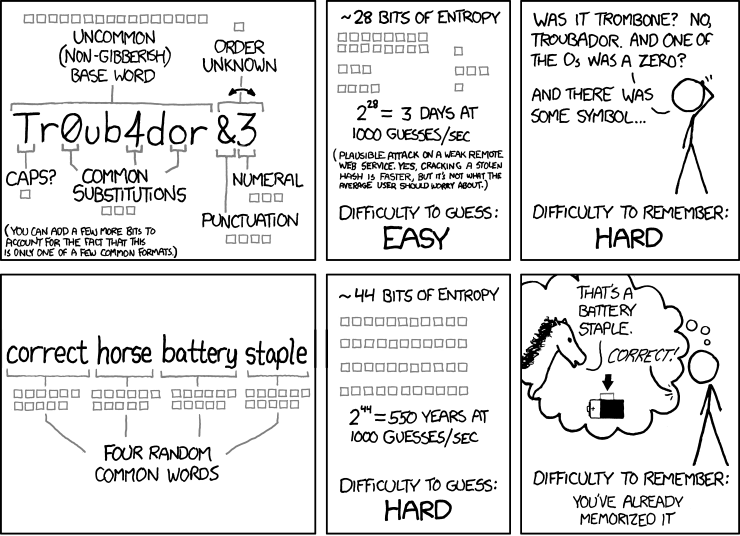
\includegraphics[width=0.7\textwidth]{xkcd.png}
    \end{figure}
\end{frame}

\begin{frame}{Passphrase generation}
    \begin{itemize}
        \item Should move away from the concept of passwords to \emph{passphrases}
        \item There are many passphrase generation techniques (DiceWare, PAO method, Schneier's Method, etc.)
        \item Recommend approach similar to xkcd. Additionally use uncommon words!
        \item Lists online of most common English words
        \item Don't use words or phrases that are meaningful to you
    \end{itemize}
\end{frame}

\begin{frame}{Password managers}
    \begin{itemize}
        \item Never reuse passwords
        \item Password managers provide an easy way to acheive this
        \item LastPass, 1password, KeePass, KeePassX
        \item With password managers the emphasis is on setting a secure master password
    \end{itemize}
\end{frame}

\begin{frame}{Strong bois}
    \begin{itemize}
        \item neon meat dream of an octafish
        \item murmuration cacophany
        \item phizzwizzwards quogwinkle
    \end{itemize}
\end{frame}

\begin{frame}{Expectations vs. reality}
    \begin{figure}
        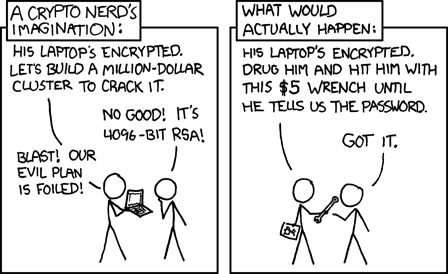
\includegraphics[width=0.85\textwidth]{security.png}
    \end{figure}
\end{frame}

\begin{frame}{Take home points}
    \begin{enumerate}
        \item Hash functions have uses in encryption and message authentication
        \item Hashed passwords can be cracked using specialist software
        \item Password managers help improve security
    \end{enumerate}
\end{frame}

\begin{frame}
    \tikz[remember picture,overlay] \node[opacity=0.3,inner sep=0pt] at (current page.center){
\includegraphics[width=\paperwidth,height=\paperheight]{thatsall.jpg}};
\end{frame}

\end{document}
